\section{First Appearance}

Continuing an approach of \textcite{roy2000}, in the following, the timing of first (and last) appearance per year is analysed. Here, the term \enquote{appearance} refers to the earliest (and latest) insect count in the recordings of a single year. In the previously mentioned publication, the authors used data recordings from the \textit{British Butterfly Monitoring Scheme} for the years 1976 to 1998 collected at over 100 sites. Among other things, they found a significant temporal shift to earlier mean first appearances in 13 out of 35 species analysed. 

In order to identify linear trends in the Fringilla dataset, a least-squares regression is applied on first appearance with year as the explanatory variable. One of the fitted models is exemplarily plotted in \cref{fig:io-linregress}. The statistical parameters of all regressions are summarized in \cref{tab:stats} of \cref{appendix}. It turns out that three species show a significant temporal trend towards earlier appearance: \textit{V. atalanta}, \textit{I. io} and \textit{P. c-album}. However, the data does not reveal a significant relationship for delayed last appearance in recent years for any species.

\begin{figure}
	\centering
	\includegraphics[width=0.9\linewidth]{"figs/Inachis io_linregress"}
	\caption{\textit{Top:} Total count of \textit{I. io} for the years 1998 to 2020, two outbreaks are visible. \textit{Bottom:} Linear regression on first (orange) and last (green) appearance. Note that the \textit{y}-axis is in days since Jan 1st of the respective year.}
	\label{fig:io-linregress}
\end{figure}

Proceeding, it would be of interest to relate climate variables to first appearance and investigate the underlying driving factors for the observed change in phenology. As the Fringilla data already includes temperature records, analysing the influence of temperature on first appearance immediately suggests itself.

\subsection{Temperature Records}

The Fringilla data includes the daily maximum temperature \parencite{shapoval2012}, however, due to the large number of missing values in early years as well as during the winter months (no monitoring from November to April), comparing the records to and eventually using other sets of temperature data is advisable. A potential replacement dataset might be the \textit{Climate Research Unit gridded Time Series} (CRU TS), covering all land domains (except Antarctica) on a \ang{0.5} latitude by \ang{0.5} longitude grid. This dataset is further discussed by \textcite{harris2020}.
As \cref{fig:annual-mean-tmp} illustrates, the temperature data displays contradictory behaviour: While---speaking of overall trends---the temperature recordings from Fringilla decrease, the annual mean temperature computed from CRU TS becomes warmer. 

\begin{figure}[H]
	\centering
	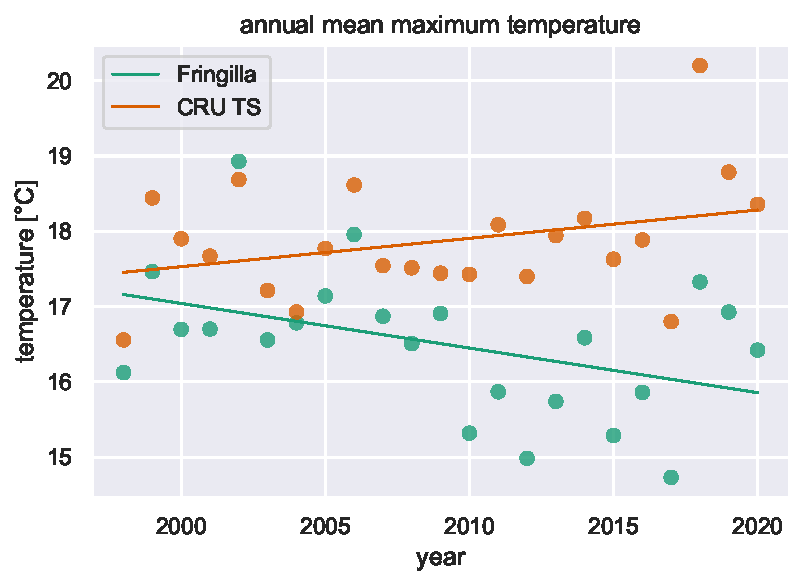
\includegraphics[width=0.9\linewidth]{figs/annual-mean-tmp-comparison}
	\caption{Comparison of the annual mean maximum temperature computed from the Fringilla dataset and CRU TS. Besides the data points, a linear fit is plotted. The annual mean is computed on the closed interval from 1st April to 31st October.}
	\label{fig:annual-mean-tmp}
\end{figure}

